\RequirePackage{mmap}
\documentclass[12pt]{article}
\usepackage[utf8]{inputenc}
\usepackage{geometry}
\geometry{
  margin=1in,
}
\usepackage{amsmath,amsthm,amssymb, listings, color}
\usepackage{mathtools}
\usepackage{changepage}% http://ctan.org/pkg/changepage
\usepackage{enumitem}
\usepackage{csquotes}
\usepackage{fancyhdr}
\usepackage[T1]{fontenc}
\usepackage{titlesec}
\usepackage[absolute]{textpos}
\usepackage[hidelinks]{hyperref}
\usepackage{fontspec}
\setmainfont{Latin Modern Roman}
%% \usepackage{setspace}
%% \doublespacing

\newcommand\defeq{\stackrel{\mathclap{\normalfont\mbox{\scriptsize def}}}{=}}
\newtheorem{theorem}{Theorem}[section]
\newtheorem{corollary}{Corollary}[theorem]
\newtheorem{lemma}[theorem]{Lemma}
\newtheorem{innercustomgeneric}{\customgenericname}
\providecommand{\customgenericname}{}
\newcommand{\newcustomtheorem}[2]{%
  \newenvironment{#1}[1]
  {%
   \renewcommand\customgenericname{#2}%
   \renewcommand\theinnercustomgeneric{##1}%
   \innercustomgeneric
  }
  {\endinnercustomgeneric}
}

\newcustomtheorem{customthm}{Theorem}
\newcustomtheorem{customlemma}{Lemma}
\newcustomtheorem{customdef}{Definition}

\setlength{\parindent}{0.25in}
\setlength{\parskip}{0.5em}

\newif\ifextra
\extrafalse

\title{}

\pagenumbering{arabic}

\begin{document}
\pagestyle{fancy}
\fancyhf{} % sets both header and footer to nothin
\cfoot{\thepage}
\renewcommand{\headrulewidth}{1pt}
\lhead{\fontsize{10}{12} \selectfont CSE 599: Convex Optimization and Geometry (Prof. Yin Tat Lee)\\\textbf{\emph{Q\&A with the Professor}} }
\rhead{\fontsize{10}{12} \selectfont Kaiyu Zheng\\ \today}

Disclaimer: I didn't take enough notes during the discussion. The answers are written based on my memory of his thought process. If there is a problem, please point out.

\begin{enumerate}
\item \textbf{Question:} I don't understand why the intersection of half spaces (resulting in convex set $K$) is expressed in the following form:
  \begin{equation}
    K = \bigcap_{\theta\in\mathbb{R}^n}\{x: \theta^Tx \leq \max_{y\in K} \theta^Ty\}
  \end{equation}
  \textbf{Answer:} Inside the set notation, $\theta$ is fixed. And because $\theta$ can be arbitrary from $\mathbb{R}^n$, you can always find a half space that covers $K$. See Figure \ref{fig:halfspace}.
  \begin{figure}[h]
    \centering
    \includegraphics[scale=1]{figs/halfspace}
    \caption{Example region $\{x: \theta^Tx\leq\max_{y\in K}\theta^Ty\}$ to be intersected with (dashed)}
    \label{fig:halfspace}
  \end{figure}

\item \textbf{Question:} I have a proof for theorem (exercise) ``the sublevel set $\{f(x)\leq t\}$ is convex''.
  \begin{proof}
    Given convex function $f$, Show $S=\{f(x)\leq t\}$ is convex. Let $x_1,\cdots,x_n\in S$. Then we have $f(x_i)\leq t_i$ for some $t_i\in\mathbb{R}$. Let $\lambda_1,\cdots,\lambda_n\in\mathbb{R}$ such that $\sum_{i}\lambda_i=1$. And let $x=\sum_{i}\lambda_ix_i$, and $t=\sum_{i}\lambda_it_i$. Then,
    \begin{align}
      f(x)=f(\sum_i\lambda_{i}x_i)&\leq\sum_i\lambda_if(x_i)\\
      &\leq \lambda_it_i = t
    \end{align}
    So $f(x)\in t$. Therefore, $x\in S$. Therefore, $S$ is convex.
  \end{proof}
  Is it correct to you?\\
  \textbf{Answer:} Yes.

\item \textbf{Question:} In the proof for the first direction of $\nabla^2f(x)\succeq 0\forall x\in\mathbb{R}^2\Leftrightarrow f$ is convex, it starts with $g(t)=f(tx+(1-t)y)$ for any $x,y\in\mathbb{R}^n$. Then, it goes:
  \begin{align}
    g(t) &= g(0) + \int_{0}^tg'(s)ds\\
    &= g(0) + tg'(0) + \int_{0}^t\int_0^sg''(u)duds\\
    &= ...
  \end{align}
  How did this expansion work?\\
  \textbf{Answer:} It's just according to:
  \begin{equation}
    f(s)-f(t)=\int_{s}^tf'(v)dv
  \end{equation}
  and rearranging.

\item \textbf{Question:} At the beginning of the notes on cutting plane methods that shows the minimizer $x^*$ lies in a half space, one statement says, ``Namely, $x^*$ lies on a half space with its normal $-\nabla f(x)$.'' I don't understand why there is a negative sign. It seems to me that it is not necessary, because the definition of half space is:
  \begin{equation}
    H^{(k)}\defeq\{x\in\mathbb{R}^n \text{ such that } \nabla f(x^{(k)})^T(x-x^{(k)})\leq 0\}
  \end{equation}
  does not have the negative. \\
  \textbf{Answer:} I will check my notes. My own answer: See Figure \ref{fig:cutting} and compare with Figure \ref{fig:halfspace}. Remember that the gradient vectors actually should point out of the page.

  \begin{figure}[h]
    \centering
    \includegraphics[scale=0.5]{figs/cutting}
    \caption{Half space containing the minimizer after one iteration of the cutting plane method.}
    \label{fig:cutting}
  \end{figure}

\item \textbf{Question:} I read somewhere else that the matrix expression for an ellipsoid is:
  \begin{equation}
    E\defeq \{x\in\mathbb{R}^n|(x-c)^TA(x-c)\}
  \end{equation}
  where $A=U\Sigma^2U^T$ \cite{pope2008algorithms}. Why did you have inverse $A^{-1}$ in your equation for ellipsoid (In section 2.2 of notes 2)?\\
  \textbf{Answer:} Because then there is no inverse in the equations for $x^{(k+1)}$, $A^{(k+1)}$, and $\hat{g}$.

\item \textbf{Question:} What is $\{a_i\}$?\\
  \textbf{Answer:} It is just a set of points. $a_i$ is a vector.

\item \textbf{Question:} Can you explain the proof for Lemma 2.3.3 (in notes 2)? The lemma goes:
  \begin{customlemma}{2.3.3}
    For any convex function $f$, we have $f^{**}=f$.
  \end{customlemma}
  Recall that the definition of convex conjugate is:
  \begin{customdef}{2.3.2}
    For any convex function $f$, we define the convex conjugate
    \begin{equation}
      f^*(\theta)\defeq \max_x\theta^Tx-f(x)
    \end{equation}
  \end{customdef}

  \textbf{Answer:} ``By the reduction via epigraph'' means consider the epigraph of $f$. To see why the theorem ``every convex function is the supremum of affine function'' is true, consider the example in Figure \ref{fig:supremum}. In this figure, we essentially have
  \begin{equation}
    f=\max_x(\{a_1x+b_1, a_2x+b_2\})
  \end{equation}
  This can be written more precisely (or safely in general) as:
  \begin{equation}
    f=\sup_{a_1,a_2}(\{a_1x+b_1, a_2x+b_2\})
  \end{equation}
  This literally means the convex function $f$ is the supremum of affine functions $a_1x+b_1$ and $a_2x+b_2$. The reason it is safer to use supremum than maximum is because, for example, $\sup_{x\in[0,1)}=1$, but $\max_{x\in[0,1)}$ does not exist.
  \begin{figure}[h]
    \centering
    \includegraphics[scale=0.4]{figs/supremum}
    \caption{Every convex function is the supremum of (some) affine functions.}
    \label{fig:supremum}
  \end{figure}    
  Therefore, for convex functions $\theta^Tx-b$, we have $f(x)\geq\theta^Tx-b=\sup_{\theta}(\theta^Tx-b)$ for all $x$. Rearranging the terms, we get $b\geq\theta^Tx-f(x)=\max_x({\theta^Tx-f(x)})$. Recall that the definition of $f^*$ (see above), then we can  substitute it in and get
  \begin{equation}
    f(x)\geq\theta^Tx-b=\sup_{\theta}(\theta^Tx-f^*(\theta))
  \end{equation}


\item \textbf{Question:} How do you go from the above to $f^{**}=f$?
  \textbf{Answer:} Didn't understand.

\item \textbf{Question:} How to intuitively understand convex conjugate? How to draw it?
  \textbf{Answer:} Didn't ask.

\item \textbf{Question:} What is an oracle?
  \textbf{Answer:} It is basically something that can produce an output by some rule given some input. It should be implemented as a program specific to the problem you are solving.
  
\end{enumerate}


\bibliography{references}
\bibliographystyle{plain}

\end{document}
